
\begin{Exercice}[10 minutes]\textbf{Maxim}
Quel est l'avantage principal d'un langage compilé ?
\mcqlist{Plus facile à corriger, Exécution plus rapide, Plus simple à écrire que les autres langages, Indépendant du système d’exploitation}
\begin{solution}
Option B.
\end{solution}
\end{Exercice}

\begin{Exercice}[10 minutes]\textbf{Maxim}
    Quelle est la différence entre un compilateur et un interpréteur ?
    \mcqlist{Le compilateur traduit le code au moment de l’exécution et l’interpréteur traduit le code avant l’exécution,
    Le compilateur traduit le code avant l’exécution et l'interpréteur traduit le code au moment de l’exécution,
    Les deux font exactement la même chose,
    Le compilateur n’est utilisé que pour les systèmes Unix}

    \begin{solution}
        Option B. 
    \end{solution}
\end{Exercice}

\begin{Exercice}[10 minutes]\textbf{Léa}

Voici la visualisation de vos dossiers (exemple: Dans le dossier Cours il y a un dossier Cours\_1):

\begin{figure}[h!]
\begin{tikzpicture}[scale=1.6,
    every node/.style = {draw=black, thick, anchor=west},
    selected/.style = {draw=OliveGreen, fill=green!30},
    file/.style = {draw=blue, fill=cyan!30},
    optional/.style = {dashed, fill=gray!50},
    grow via three points={one child at (0.5,-0.7) and two children at (0.5,-0.7) and (0.5,-1.4)},
    edge from parent path={(\tikzparentnode.south) |- (\tikzchildnode.west)}
]
\node [selected] {\faFolder[regular] /User}
child { 
    node [selected] {\faFolder[regular] /Cours}
    child { 
        node [selected] {\faFolder[regular] /Cours\_1}
        child { 
            node [file] {\faFile[regular] Slides\_1.pdf}
        }
    }
}
child [missing] {}
child [missing] {}
child { 
    node [selected] {\faFolder[regular] /TPs}
    child { 
        node [selected] {\faFolder[regular] /Solutions}
    }
    child { 
        node [file] {\faFile[regular] tp1.py}
    }
    child { 
        node [file] {\faFile[regular] tp1.java}
    }
}
child [missing] {}
child [missing] {}
child [missing] {}
child { 
    node [selected] {\faFolder[regular] /Documents}
}
child { 
    node [selected] {\faFolder[regular] /Photos}
};
\end{tikzpicture}
\end{figure}
\FloatBarrier

Vous ouvrez un terminal et vous êtes dans le dossier TPs, qu'est ce qui va être affiché dans le terminal si vous tapez \texttt{ls} sur un système d'exploitation UNIX (Linux/MacOS) (on écrit tout à la même ligne par souci de concision):

\mcqlist{\texttt{Solutions tp1.py tp1.java}, \texttt{TPs Solutions tp1.py tp1.java}, \texttt{Cours Cours\_1 Slides\_1 TPs Solutions tp1.py tp1.py Photos Documents}, \texttt{tp1.py tp1.java}}

\begin{solution}
Option A. 
\end{solution}
\end{Exercice}

\begin{Exercice}[10 minutes]\textbf{Léa}
Vous êtes toujours dans le dossier TPs et vous voulez aller dans le dossier Solutions, quelle commande tapez vous dans le terminal?
\mcqlist{\texttt{rm Solutions},\texttt{mv Solutions}, \texttt{cd Solutions},\texttt{mkdir Solutions}}
\begin{solution}
Option C. 
\end{solution}
\end{Exercice}

\begin{Exercice}[10 minutes]\textbf{Sean}


Vous vous trouvez dans un dossier qui contient deux sous-dossiers : \faFolder[regular] \textcolor{blue}{python} et \faFolder[regular] \textcolor{blue}{java}.
\begin{itemize}
    \item[$\bullet$] Le dossier \textcolor{blue}{python} contient un unique fichier nommé \textcolor{green}{hello.py}.
    \item[$\bullet$] Le dossier \textcolor{blue}{java} contient un unique fichier nommé \textcolor{green}{hi.java}.
\end{itemize}

\textbf{(a)} Quelle(s) commande(s) devez-vous taper dans le terminal, ouvert depuis le dossier \textbf{parent} de \textcolor{blue}{python}, pour exécuter le programme \textit{hello.py} ? \\ 

\textbf{(b)} Après avoir exécuté les commandes de la question (a), quelles commandes faut-il saisir pour compiler puis exécuter le programme \textit{hi.java} situé dans le dossier \textit{java} ? \\ 

\textbf{(c)} Après avoir exécuté le programme \textit{hi.java}, si vous vous placez dans le dossier \textit{java} et que vous tapez la commande \textbf{ls}, quelle sera la sortie affichée dans le terminal ?

\begin{solution}
\textbf{a.} \texttt{python python/hello.py} \newline 
\textbf{b.} \texttt{javac java/hi.java} ensuite \texttt{java java/hi.javac}. Alternativement, \texttt{javac java/hi.java \&\& java java/hi.javac} \newline 
\textbf{c.} \\
\texttt{hi.javac} \newline \texttt{hi.java}  
\end{solution}
% \vspace{1em}
% \noindent\rule{\textwidth}{0.4pt}

% \subsection{Solution}

% \textbf{(a)}

% \begin{lstlisting}[language=bash]
% cd python
% python hello.py
% \end{lstlisting}

% Alternative en une seule commande :

% \begin{lstlisting}[language=bash]
% python python/hello.py
% \end{lstlisting}

% \noindent{\color{Maroon}\rule{4cm}{2pt}}

% \textbf{(b)}

% \begin{lstlisting}[language=bash]
% cd ..
% cd java
% javac hi.java
% java hi
% \end{lstlisting}

% Alternative si vous êtes toujours dans le dossier parent de python :

% \begin{lstlisting}[language=bash]
% cd java
% javac hi.java
% java hi
% \end{lstlisting}

% \noindent{\color{Maroon}\rule{4cm}{2pt}}

% \textbf{(c)}

% La sortie affichée sera :

% \begin{lstlisting}
% hi.java
% hi.class
% \end{lstlisting}

\end{Exercice}


\begin{Exercice}[10 minutes]\textbf{Amina}
La commande \texttt{pwd} permet de:
\mcqlist{Afficher le chemin absolu du répertoire courant, Supprimer le répertoire courant, Créer un nouveau fichier, Afficher la liste des fichiers dans le répertoire courant.}
\begin{solution}
Option A. 
\end{solution}
\end{Exercice}

\begin{Exercice}[10 minutes]\textbf{Amina}
Parmi ces commandes, laquelle permet de créer un nouveau répertoire ?
\mcqlist{\texttt{ls}, \texttt{cd}, \texttt{mkdir}, \texttt{pwd}}
\begin{solution}
\texttt{mkdir}
\end{solution}
\end{Exercice}

\begin{Exercice}[10 minutes]\textbf{Aurore}
Voici la ligne de commande d'un terminal sur une machine MacOS/Linux (à gauche) et Windows (à droite).

\begin{figure}[h!]
    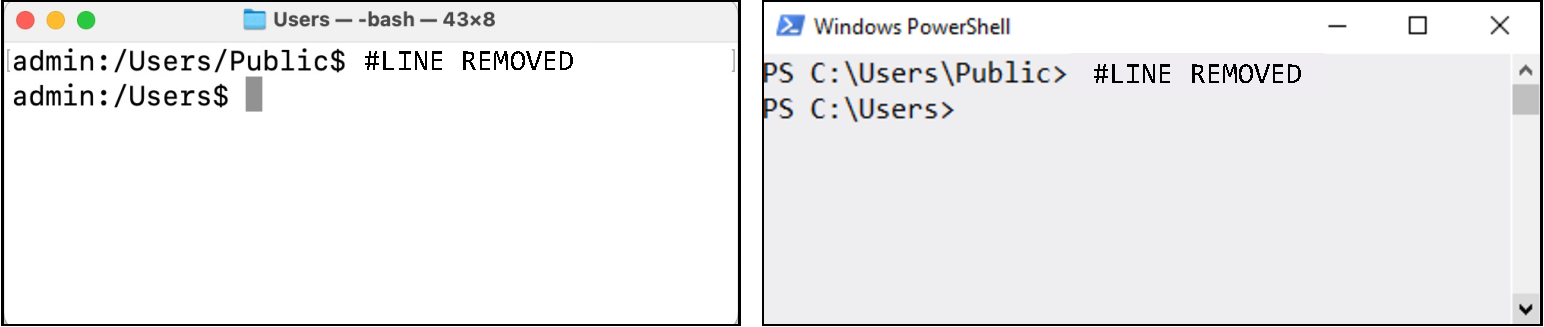
\includegraphics[width = \textwidth]{res/bashq21.pdf}
\end{figure}

Quelle commande a été passée (\#LINE REMOVED)?

\mcqlist{\texttt{dir}, \texttt{cd Users}, \texttt{cd ..}, \texttt{ls}}
\begin{solution}
\texttt{cd ..}
\end{solution}
\end{Exercice}


\begin{Exercice}[10 minutes]\textbf{Aurore}
Laquelle des affirmations suivantes est fausse?
\mcqlist{Un langage compilé est traduit ligne par ligne au moment de l'exécution, 
{En Java, l'étape de compilation et d'interprétation sont séparées}, 
Un langage interprété est plus lent à exécuter, 
Les langages Python et Java nécessitent les deux une traduction en bytecode, 
Toutes les affirmations sont correctes}

\begin{solution}
Option A. 
\end{solution}
\end{Exercice}
